\documentclass[12pt, dvipdfmx, pdfversion=1.5]{jarticle}
\usepackage{ilsfonts}    % 卒論スタイルで使うフォントの定義
\usepackage{ilssoturon}  % 卒論スタイル宣言
\usepackage[dvips]{graphicx} % グラフィクスの利用宣言
\usepackage{amsmath,amssymb} % 数学記号などの利用宣言
\usepackage{bm}  % 太字数式文字の利用に関する宣言
%\usepackage{slashbox} % 表に斜線を入れる(不要かも)
%\usepackage[dvips]{graphicx,psfrag} % 図に数式を使うときに用いる(別の方法がおすすめ)
%\usepackage[dvipdfmx]{graphicx} %図
% ハイパーリンクを作るためのパッケージだが,pdf viewerによってはハイパーリンクの枠が描画されたまま出力されるので,基本的には使用しない
%\usepackage[dvipdfmx]{hyperref}
%\usepackage{pxjahyper} % 日本語しおりを作るためのパッケージ

\usepackage{here} %図を強制的に表示させる

%ここからソースコードの表示に関する設定
\usepackage{listings,jlisting}
\lstset{
  basicstyle={\ttfamily},
  identifierstyle={\small},
  commentstyle={\smallitshape},
  keywordstyle={\small\bfseries},
  ndkeywordstyle={\small},
  stringstyle={\small\ttfamily},
  frame={tb},
  breaklines=true,
  columns=[l]{fullflexible},
  numbers=left,
  xrightmargin=0zw,
  xleftmargin=0zw,
  numberstyle={\scriptsize},
  stepnumber=1,
  numbersep=1zw,
  lineskip=-0.5ex
}

\年度{2023年度} % 以下は論文表紙に出力される内容
\提出日{2024年1月xx日}
\研究者{2031133 &増田 瑞樹}
\論文題目{WANNにおける活性化関数の慎重な選択}

\begin{document} % ここから論文本体
\卒論表紙 % これで数式が出る

% 正しく目次を出力するためには tex コンパイルを2回連続でかけること
\pagenumbering{roman} % 目次のページ番号はローマ数字

\tableofcontents % 目次を出す命令
\clearpage % 改ページ

\pagenumbering{arabic} % ページ番号をアラビア数字になおす

\section{はじめに}
生物学における先天的能力(Precociality)とは,動物が生まれた瞬間からすでに持っている能力のことである.例えば,トカゲやヘビは生まれ持って捕食者から逃れる能力を有している.また,アヒルは孵化後すぐに泳いだり食事をすることができ,七面鳥は一度も見たことがない捕食者を視認するすることができる.これは,動物の脳は高度に構造化された状態で生まれ,その構造はゲノムに記憶されていることを意味する.Zadorは生物学的な学習について『動物の行動の多くは生得的なものであり学習によって生じるものではない.動物の脳はAI研究者が思い描くようななんでも学べる汎用的な学習アルゴリズムを備えた白紙の状態ではない.』と強調している\cite{先天的能力}.\\
Weight Agnostic Neural Networks(WANN)は,2019年にAdam GaierとDavid Haによって発表されたシナプス荷重に依存しないネットワークの探索アルゴリズムである\cite{WANN}.WANNは,NEAT\cite{NEAT}をベースに作られており,どのようなシナプス荷重においてもタスクを解ける性質をもつネットワーク,つまり構造自体にタスクを解く機能が備わっている.これは遺伝的アルゴリズム\cite{遺伝的アルゴリズム}を用いたNeuro-Evolution\cite{NE}の手法から実現できる.\\
WANNの個体変異の1つに,ノードの活性化関数の変更が行われる.隠れ層からランダムに選択されたノードの活性化関数は現在採用されている以外の活性化関数に同様に確からしく選択される.これは探索後期において,それまでの良かったノードの出力を反転させてしまう懸念がある.\\
本論文では,活性化関数を変更する際の確率を関数同士の距離関数が小さいほど選ばれやすいようにする手法を提案する.距離関数が小さいことは,関数同士が似ているを意味し,活性化関数の変更により出力の大きな変更が起こりにくくなる.距離関数には0付近の活性化関数同士の出力の差を積分と,実際にその個体が体験した入力ノードから推測できる該当ノードの出力の差の合計を採用する.\\
実験では \textbf{ここから追加} %はじめに
\clearpage

\section{ニューラルネットワーク}
\subsection{ニューラル素子}
人間を含む生命の脳を構成する神経細胞はニューロンと呼ばれ,人間の脳には140億個のニューロンがありそれぞれのニューロンは平均約8,000個のシナプスを持つとされている.ニューラルネットワークのノードはニューロンをモデルとし,計算機上でニューロンをシミュレートできるよう設計されている.
\\ \textbf{ここに図} \\
ここでは,素子への $ N $ 個の入力 $ S_1, S_2, ..., S_N $ に対して各々の重み $ w_1, w_2, ..., w_N $ となっている.この素子は入力からバイアス $ b $ を足した値を活性化関数 $ f $ の入力とし,活性化関数の出力をノードの出力 $ z $ とする.

\begin{equation}
    z = f(\sum_{i=1}^N S_i + b)
\end{equation}

主に活性化関数 $ f $ には次のような関数を用いる.

\begin{enumerate}
    \item tanh関数
    \begin{equation}
        f(x) = \frac{e^{x} - e^{-x}}{e^{x} + e^{-x}}
    \end{equation}

    \item ReLU関数
    \begin{equation}
        f(x) = 
        \begin{cases}
        x & (x > 0)\\
        0 & (x \leq 0)
        \end{cases}
    \end{equation}
\end{enumerate} %ニューラルネットワーク
\clearpage

\section{遺伝的アルゴリズム}
遺伝的アルゴリズム(GA)とは,適用範囲の非常に広い,生物の進化を模倣した学習的アルゴリズムである\cite{遺伝的アルゴリズム}.すなわち何万年,何億年もかけて生物の特徴が進化してきたような遺伝的法則を光学的な手法にモデル化し,また参考にしてタスクを解くものである.自然界における生物の進化過程においては,ある世代を形成している個体の集合,すなわち個体群の中で環境に適している個体が高い確率で生き残り,生き残った個体は交叉や突然変異によって次の世代の個体群が形成される.

\subsection{本論文における基本的動作}
本論文において,新しく個体を形成する際に交叉は使用しない.以降本論文で用いる遺伝的アルゴリズム変則GAと呼ぶ.図は変則GAの動作を流れを表している.

\begin{figure}[h]
    \begin{center}
        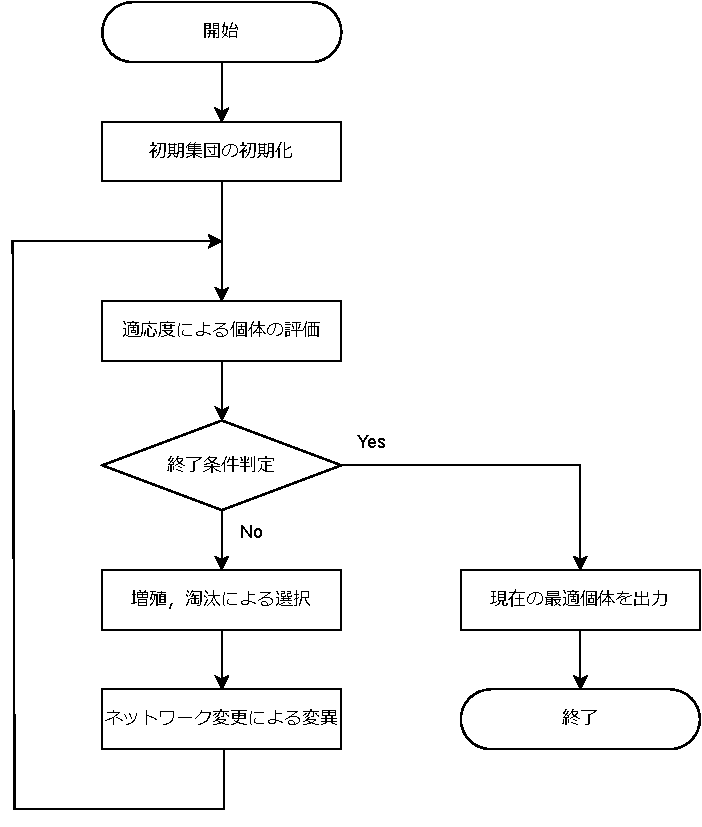
\includegraphics[scale=0.8]{img/expga.pdf}
        \caption{変則GAの概要}
    \end{center}
\end{figure}


\begin{enumerate}
    \item 初期化 \\
    ランダムな性質を持つ個体を $ N $ 個生成し,初期世代の個体群を設定する.

    \item 評価 \\
    各個体についてタスクを解かせ,その進捗により適応度を測定する.

    \item 終了判定 \\
    終了条件を満たしていれば,その時に得られる最適個体を問題の準最適解として出力する.

    \item 選択 \\
    各個体に対応する適応度により並べ替え,適応度の低い個体は淘汰され,適応度の高い個体は増殖する.

    \item 変異 \\
    設定された突然変異の設定により変異を行い,新しい個体群を生成する.変異を行った後の個体群は次世代の個体群として再度評価される.
\end{enumerate}

終了判定には最良個体の適応度や個体群の平均の適応度を参照する場合が多いが,本論文ではあらかじめ設定した世代数を超えたときにのみ終了判定が真になり,プログラムは終了する.また,変異をする過程でエリート保存選択を実行する.これは非常に優れた個体は変異をする前の状態のほうが変異をした後の状態よりも優れている見込みが大きいことから,個体に対して変異を行わず,全く同じ状態の個体を次世代に残す手法である.エリート保存選択は,むやみに変異をして優良個体の遺伝子を破壊しないことにつながる.

\subsection{ルーレット選択}
ルーレット選択は,個体群の中の各個体の適応度とその総計を求めて,適応度の総計に対する各個体の割合を選択確率として個体を選択するという基本的な考えに基づいている\cite{遺伝的アルゴリズム}.すなわち,ルーレット選択では,個体 $ s_i $ の適応度 $ f{s_i} $ と個体群の総計を求め,個体 $ s_i $ が選択される確率を

\begin{equation}
    P_i = \frac{f(s_i)}{\sum^N_{j=1} f(s_j)}
\end{equation}

として個体の確率的に選択する.このようなルーレット選択のアルゴリズムは,次のように要約される.

\begin{enumerate}
    \item 世代 $ t $ の個体群 $ X(t) $ の中の $ N $ 個の個体の適応度 $ f_i $ とその総計 $ f_{sum} = \sum^N_{i=1} f_i $ を求める.

    \item 区間[0, 1]の乱数 $ rand $ を発生させ, $ s = rand \times f_{sum} $ とする.

    \item $ \sum^k_{i=1} f_i \geq s $ となるような最小の $ k $ を求めて, $ k $ 番目の個体を世代 $ t+1 $ に生き残る個体の候補とする.

    \item 候補となる個体数が $ N $ になるまで2, 3を繰り返す.
\end{enumerate}

本論文ではルーレット選択を個体の変異先を選択する際に用いる.同じ構造を持つネットワークの,ひとつのノードの活性化関数のみを変更し,この出力が小さいほど $ f_i $ が大きいことになる.
 %遺伝的アルゴリズム
\clearpage

\section{Weight Agnostic Neural Networks}

\begin{figure}[h]
    \begin{center}
        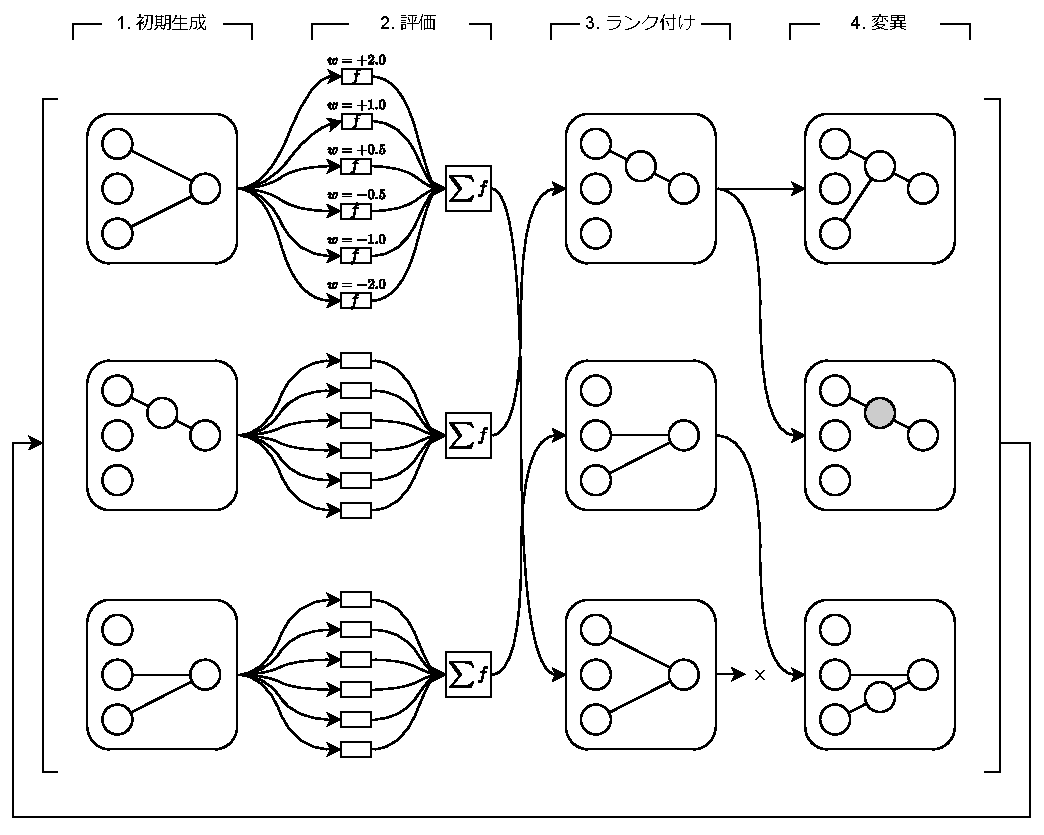
\includegraphics[scale=0.8]{img/expwann.pdf}
        \caption{WANNsの概略図}
    \end{center}
\end{figure}

Weight Agnostic Neural Networks(WANNs)は,2019年にAdam GaierとDavid Haによって発表されたニューラルネットワークの構造探索アルゴリズムである\cite{WANN}.WANNは,NEAT\cite{NEAT}をベースに作られており,これは遺伝的アルゴリズム\cite{遺伝的アルゴリズム}を用いたNeuro-Evolution\cite{NE}の手法から実現できる.多くのニューラルネットワークはシナプス荷重を更新することで,ネットワークの精度を向上させているが,WANNsによって生成された個体は,ネットワーク構造自体がタスクを解く性質を持っており,どんなシナプス荷重においてもそれなりの精度でタスクを解くことができる.これは生物の先天的能力と似た性質であると言える\cite{先天的能力}.また,WANNsネットワークはそれぞれのノードが別々の活性化関数を持っている.WANNの概略図を図3に示す.WANNにおける探索は以下の動作によって実現する.

\begin{enumerate}
    \item 初期生成
    個体は最初,最もシンプルな構造を持つネットワークからなる.中間層は存在せず,入力層のうちの一部からシナプスが出力層に接続されている.

    \item 評価
    各個体に対して,ネットワーク全体の共有重みを使用してタスクを実行する.本論文では, $ -2.0, -1.0, -0.5, +0.5, +1.0, +2.0 $ の6つの共有重みを使用する.また,タスクを解く際の初期状態により優れた結果を残せずに誤った評価をしないよう,それぞれの共有重みにて4回のタスクを実行する.最終的に6つの共有重みと4回の試行から得られた24個の評価値を合計する.

    \item ランク付け
    個体をランク付けする.上位の優れた個体は変更のないまま次世代へ保存され,下位の劣った個体は淘汰される.このランク付けはネットワークの評価値とネットワークの複雑さから算出される.

    \item 変異
    個体をランクのトーナメント選択\cite{遺伝的アルゴリズム}によって選択し,変異を起こした次世代の個体として保存する.

    保存された個体は再度評価,ランク付け,変異を行い,任意の世代数まで繰り返される.
\end{enumerate}

ニューラルネットワークには,その用途を達成するために適したネットワーク構造がある.画像認識には畳み込みニューラルネットワーク(CNN),自然言語処理には再起型ニューラルネットワーク(RNN)などを用いることで全結合型ニューラルネットワークよりも少ない計算量でよりよい精度を実現することができる\cite{深層学習}.自然界においても海には魚類,陸上には哺乳類などある環境下に適した身体的特徴や先天的能力をさまざまな生物が獲得している\cite{先天的能力}.ラットは生まれてから経験したことを,少なくとも小脳皮質のシナプスを追加することによってよりよいフィードバックができるように学習する\cite{シナプス学習}.WANNsはあるタスクにおいてのみ優れた精度を持つニューラルネットワークを探索するアルゴリズムで,今までのネットワーク構造ありきのシナプス重みを重視する手法とは違い,どんな重みであっても動作するネットワーク構造に着目した手法であり,生物の基本的な性質を踏襲したものになっている.結果として,十分に世代を重ねたときの最良個体の出力は,0付近を除いたすべての共有重みを用いた際に安定している.
\begin{figure}[h]
    \begin{center}
        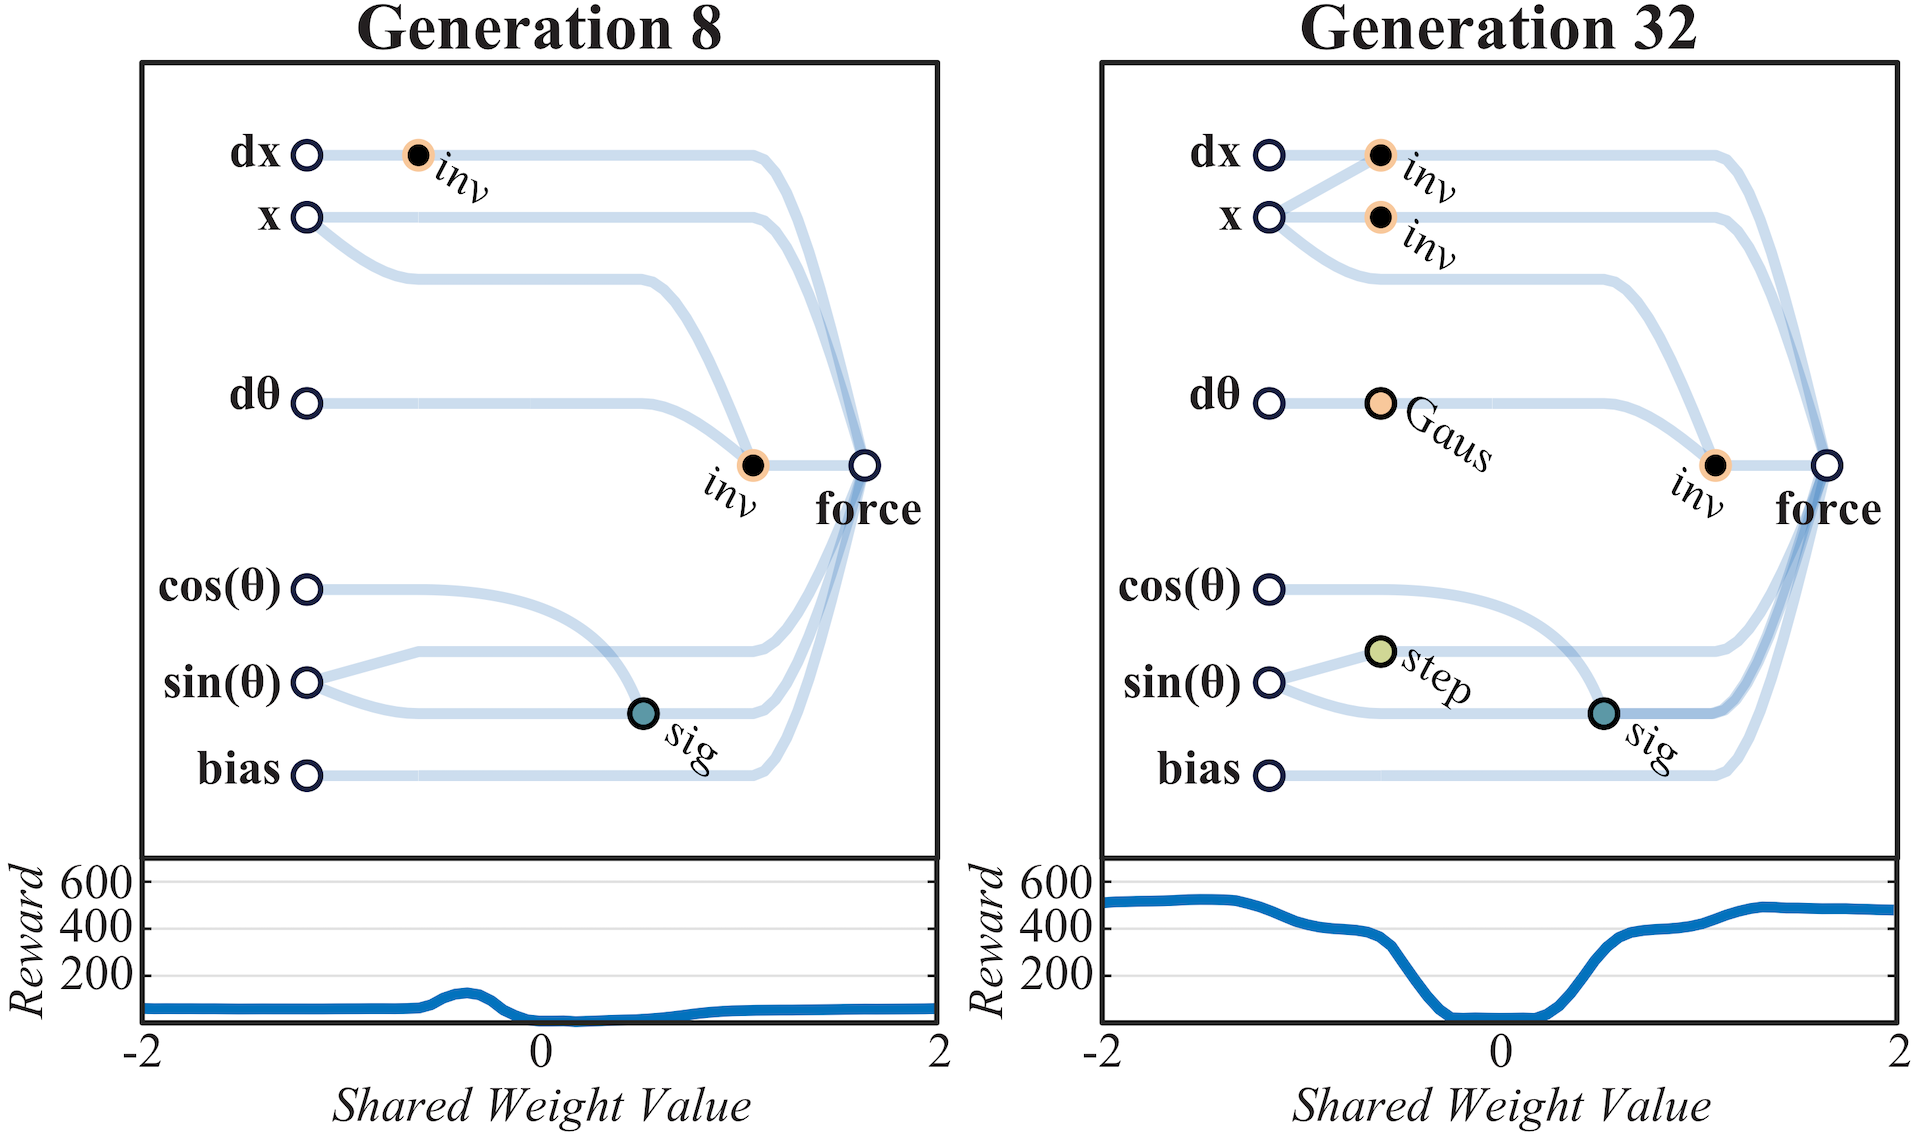
\includegraphics[width=120mm]{img/wannweight.png}
        \caption{WANNsのネットワーク構造と共有重み}
    \end{center}
\end{figure}


\subsection{変異}

\begin{figure}[h]
    \begin{center}
        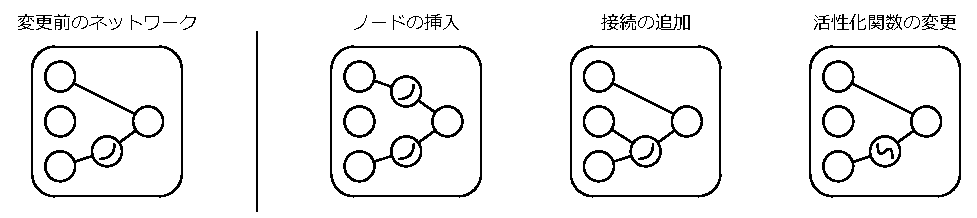
\includegraphics[scale=0.8]{img/vary.pdf}
        \caption{WANNsのネットワーク変異}
    \end{center}
\end{figure}

図に示したように,個体の変異にはノードの挿入,接続の追加,活性化関数の変更のいずれかを行い,各操作の具体的な手順は以下のようになる.

\begin{enumerate}
    \item ノードの挿入
    ネットワークの持つひとつの接続をランダムに選択し,接続の途中にひとつのノードを追加する.この時の活性化関数はランダムに選択される.

    \item 接続の追加
    接続を持たないふたつのノードを選択し,それらをつなぐ接続を追加する.

    \item 活性化関数の変更
    ネットワークの持つ中間層のノードを選択し,そのノードの活性化関数を変更する.活性化関数は現在選択されている関数以外の関数がランダムに選択される.このときの活性化関数はlinear, step, sin, cosine, Gaussian, tanh, sigmoid, inverse, absolute value, ReLUを利用する.
\end{enumerate} %WANN
\clearpage

\section{提案手法}
既存手法の問題点として,ランダムな活性化関数の変更が挙げられる.探索後期において良いノードの出力の個体が生まれたとしても,例えば良いノードの活性化関数をlinear関数 $ f(x) = x $ からinverse関数 $ f(x) = -x $ に変更されてしまうと,ノードの出力は反転されてしまう.ネットワークの一部の構造化された部分の出力の大小は,同符号であれば出力層に大きな変化をもたらさないが,出力が0より大きいか小さいかは,ネットワークの出力は大きく変わることが知られている\cite{WANN}.\\
提案手法ではこれの問題を緩和するために,活性化関数の慎重な選択について言及する.2つの活性化関数の距離を計算し,距離が小さければ小さいほど変更先の活性化関数として選択されやすくなる.

\begin{figure}[h]
    \begin{center}
        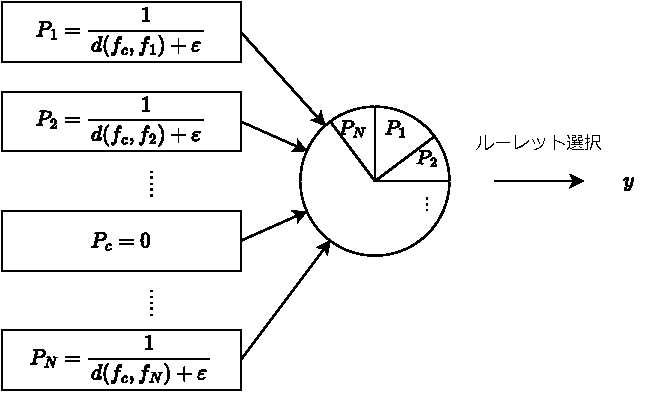
\includegraphics[scale=0.8]{img/exppropose.pdf}
        \caption{提案手法の概略図}
    \end{center}
\end{figure}

\begin{equation}
    P_{i} =  \begin{cases} \dfrac{1}{d(f_{c}, f_{i}) + \epsilon_{n} } \qquad (i \neq c) \\ 0 \qquad (i = c) \end{cases}\\
\end{equation}
\begin{equation}
    \epsilon_{n} = s * \epsilon_{n-1} \\
\end{equation}

\begin{table}[h]
    \caption{変数の説明}
    \centering
    \begin{tabular}{cl}
        \hline
        変数  & 意味 \\
        \hline \hline
        $P_{i}$               & $c$から$i$へ活性化関数IDが変更される見込み \\
        $d(f_{c}, f_{i})$     & 活性化関数が$c$と$i$の距離                 \\
        $f_{i}$               & IDが$i$の活性化関数                        \\
        $i$                   & 活性化関数ID                               \\
        $c$                   & 現在の活性化関数ID                         \\
        \hline
    \end{tabular}
\end{table}

まず現在の活性化関数 $ f_c $ と,すべての活性化関数との距離を計算する.この時の距離が小さいことは両者の関数が似ていることを意味し,距離の短い関数への変更は既存手法の問題点である出力の反転を防ぐ.距離が小さければ小さいほど選択されやすくするため,距離と $ \epsilon $ の和の逆数をルーレット選択の材料とする. $ \epsilon $ が大きくなると,ルーレット選択によって選ばれる確率はランダムに近くなる. $ \epsilon $ は探索初期においては,良いノードの出力を持つ個体が少ないことから,良い出力の個体を反転させてしまうデメリットより,悪い出力の個体を反転させるメリットの方が大きいと考え,探索初期の $ \epsilon $ は大きく,探索後期の $ \epsilon $ は小さく設定する.グラフは代表的な活性化関数4種,活性化関数同士の区間積分差を用いた活性化関数の変更として選択される確率を表した例である.\\

ここに図 \\

距離関数 $ d $ については,区間積分差と,個体の経験に基づく出力差を採用する.

\subsection{活性化関数同士の区間積分差}
式(7)は関数 $ f_a $ と $ f_b $ の範囲内の出力の差を意味している.

\begin{equation}
    d(f_{a}, f_{b}) = \int^{r}_{-r} (f_{a}(x) - f_{b}(x))^{2}
\end{equation}

\begin{table}[h]
    \caption{式(8)の変数の説明}
    \centering
    \begin{tabular}{cl}
        \hline
        変数  & 意味 \\
        \hline \hline
        $d(f_{a}, f_{b})$ & 活性化関数が$a$と$b$の距離                 \\
        $f_{i}$           & IDが$i$の活性化関数                        \\
        $r$               & 関数の考慮範囲                             \\
        \hline
    \end{tabular}
\end{table}

実際にネットワークにタスクを解かせる際,ノードへの入力は0付近である場合が多いので\cite{ノード入力}, $ -r $ から $ +r $ までの関数の区間積分によって距離を定義する.区間内の入力に対して出力の差が小さいことは,活性化関数を変更してもネットワークに大きな動作の変更をもたらさないことを意味し,局所的な解を優先的に探索する.番号が $ 1 $ から $ N $ と振られている活性化関数 $ f_n $ から $ f_N $ ,現在の活性化関数が $ f_c $, $ f_n $ と $ f_c $ の距離を $ d_n $ としたときの具体的なプログラムの実装は以下のようになる.

\begin{lstlisting}[caption=区間積分差のプログラム]
for n (1 to N)
    sum = 0
    for x (-r to +r)
        sum += (activate(x, n) - activate(x, c)) ^2
    d[n] = sum
\end{lstlisting}

ネットワークで使用する活性化関数にはそれぞれIDが1-based(1からナンバリングする方式)により割り振られており,1からNまでのそれぞれの活性化関数IDに対してその関数と変更前の関数との差の2乗を変数sumに加算していく.変数xをとても小さい数ずつ増やしていき,x範囲内の合計が最終的にsumに格納され,変更前の活性化関数の出力と活性化関数IDがnの関数の出力の差を2乗をd[n]に代入する.このように求めた $ d_n $ を式(6)に代入しルーレット選択により選ばれる見込み $ P_n $ を得る.
また, $ x $ を活性化関数の入力とした出力を求める関数 activate は後述する.

\subsection{個体の経験に基づく出力差}
式(7)は関数 $ f_a $ と $ f_b $ の個体が経験したノードの入力に対する差を意味している.
\begin{equation}
    d(f_{a}, f_{b}) = \sum_{m=1}^{M}(f_{a}(in_{m}) - f_{b}(in_{m}))^2
\end{equation}

\begin{table}[H]
    \caption{変数の説明}
    \centering
    \begin{tabular}{cl}
        \hline
        変数  & 意味 \\
        \hline \hline
        $d(f_{a}, f_{b})$ & 活性化関数が$a$と$b$の距離                 \\
        $f_{i}$           & IDが$i$の活性化関数                        \\
        $M$               & ミニバッチサイズと共有重みの積             \\
        $in_m$            & ミニバッチ $m$ 回目に経験したノードに入力される値 \\
        \hline
    \end{tabular}
\end{table}

区間積分差は範囲内のすべての領域を考慮し差を求めたのに対し,個体の経験に基づく出力差では,実際に個体がタスクを実行したときに経験した入力ノードの値を利用する.ネットワークの構造に変化はないので,入力ノードの値が分かれば,ネットワーク内の全てのノードの出力を特定することができ,ネットワークの変更にあたり指定した隠れ層のノードの出力を入力ノードから計算する.このとき指定したノードの活性化関数のみ変更し,この差を2乗を加算することで,個体が経験した入力に対する出力の差の小さい活性化関数を求めることができる.領域内を満遍なく考慮する手法よりも実際の入力ノードを利用することで出現確率の高いノード入力を大きく考慮することを期待する.ミニバッチには,同じ個体であれば異なる共有重みを使用していても利用する.

\begin{lstlisting}[caption=経験入力に基づく出力差のプログラム]
out(nodeID, actID, state, weight)
    preout = 0
    connect[] = synapses where the destination is nodeID
    node = Information of node where the ID is nodeID

    if(node[Type] == input)
        preout = state[nodeID]
    
    else
        for i (0 to connect)
            newnodeID = connect[source]
            newactID = activationID[connect[source]]
            val = out(newnodeID, newactID, state[x], weight)
            preout += val
    
    prein = preout * weight[m]
    output = activate(prein, actID)
    return output

weight = [-2.0, -1.0, -0.5, +0.5, +1.0, +2.0]
for n (1 to N)
    sum = 0
    for m (0 to 5)
        for x (0 to miniBatchSize)
            sum += (out(ID, n, m, state[x]) - out(ID, c, m, state[x])) ^2
    d[n] = sum
\end{lstlisting}

1からNまでの各活性化関数に対してノードの出力の差を求める.各共有重みに対してミニバッチのうちのひとつの入力ノード情報を利用する.state[x]には個体が経験した入力ノード情報が記憶されており,今回使用するタスクBipedalWalker-v2\cite{OpenAI}では,入力層のノードは24個なので要素数24の配列となる.ノードの出力を求める関数 out には,出力を求めたいノードID,活性化関数ID,入力ノード情報,共有重みの値を入力としている.関数 out に入力された nodeID が指すノードが入力層であれば入力ノードデータを返し,隠れ層であれば目的地が nodeID であるすべてのシナプスの 出発地になっているノードに対して出発地のノードIDを newnodeID ,出発地のノードの活性化関数IDを newactID として out を再帰的に実行する.シナプスの出発地を辿り続けるといつか必ず入力層となるため, val を必ず得ることができる.最初に呼び出した out に入力した nodeID に入力される値を今までの合計と共有重みの積から計算し,関数 activate に通すことで活性化関数の出力に対応する.最終的に関数 out は nodeID の出力を返し,異なる活性化関数 n と c の差の2乗を sum に加算していく.区間積分の手法と同じく n と c の差は d[n] に代入される.ソースコード2の out(ID, n, m, state[x]) は式(9)の $ f_{a}(in_{m}) $ と同等の意味を持つ. $ x $ を活性化関数の入力とした出力を求める関数 activate は後述する.

\subsection{用いる活性化関数}
今回用いる活性化関数には,1-basedにナンバリングされ,以下の10種類を用いる.また関数への入力 $ x $ に対応する出力 $ y $ を示した数学的表現,pythonで実装した入力 x に対応する value を示す.

\begin{table}[H]
    \caption{用いる活性化関数とその式}
    \centering
    \begin{tabular}{clll}
        \hline
        ID & 関数名 & 数学的表現 & プログラム上での表現 \\
        \hline \hline
        1 & Linear & $ y = x $ & value = x \\
        2 & Step & $ y = \begin{cases}
            1.0 & (x > 0.0) \\
            0.0 & (x \leq 0)
            \end{cases} $ & \texttt{value = 1.0*(x>0.0)} \\
        3 & Sine & $ y = \sin(\pi x) $ & value = np.sin(np.pi*x) \\
        4 & Gaussian & $ y = e^{-\frac{x^2}{2}} $ & value = np.exp(-np.multiply(x, x) / 2.0) \\
        5 & Hyperbolic Tangent & $ y = \frac{e^{x} - e^{-x}}{e^{x} + e^{-x}} $ & value = np.tanh(x) \\
        6 & Sigmoid & $ y = \frac{\tanh\left(\frac{x}{2}\right) + 1}{2} $ & value = (np.tanh(x/2.0) + 1.0)/2.0 \\
        7 & Inverse & $ y = -x $ & value = -x \\
        8 &Absolute & $ y = |x| $ & value = abs(x) \\
        9 & Relu & $ y = 
        \begin{cases}
        x & (x > 0)\\
        0 & (x \leq 0)
        \end{cases} $ & value = np.maximum(0, x) \\
        10 & Cosine & $ y = \cos(\pi x) $ & value = np.cos(np.pi*x) \\
        \hline
    \end{tabular}
\end{table}

上で使用した activate 関数は,入力値と活性化関数IDとし,表に従いvalueを出力する.

\subsection{距離関数の妥当性}
提案手法では,活性化関数同士の出力の差の大きさを距離関数として表現している. \\
実数の組から実数への写像を実現する関数 $ d: \mathbb{R} \times \mathbb{R} \rightarrow \mathbb{R} $ が距離関数であるとは, $ x, y, z $ を $ \mathbb{R} $ の任意の元として,以下の条件が満たされていることを言う\cite{距離関数}.

\begin{table}[H]
    \caption{距離関数の性質}
    \centering
    \begin{tabular}{cl}
        \hline
        性質  & 定義 \\
        \hline \hline
        非負性     & $ d(x, y) \geq 0 $ \\
        同一律     & $ d(x, y) = 0 \Leftrightarrow x = y $ \\
        対称律     & $ d(x, y) = d(y, x) $ \\
        三角不等式 & $ d(x, y) \leq d(x, z) + d(z, y) $ \\
        \hline
    \end{tabular}
\end{table}

同一律については,$ d(x, x) = 0 $ とは違う意味を示していることに注意する. $ x $ と $ x $ の距離は当然0であるが, $ x $ と $ y $ が同一でない限り距離が0にはならないことを示している.つまり $ x $ と $ y $ が別のものを指しているのに関わらず距離が0になった場合,その関数dは距離関数としての性質を満たしていないことになる.これらの証明をするにあたって,2つの提案手法について確認する.式(8)と式(9)はいずれも一定の数の要素を持つ配列の,各要素同士の差を2乗したものの総和ととれる.各要素の値はどのようなものであっても距離関数を満たすため,ここでは以下のようにし証明を簡略化する.

\begin{equation}
    d(a, b) = \sum_{i=o}^{N-1}(a[i] - b[i])^2
\end{equation}

ここで $ f_{a}(x) $ や $ f_{a}(in_{m}) $ を $ a[i] $ とすることは,どのような実数に対しても関数が距離関数の性質を持つことから,そのうちの一例である $ f_{a}(x) $ や $ f_{a}(in_{m}) $ も例外でなく距離関数の性質を持つと導くことができる.以下は同じ要素数の配列に任意の実数を代入したときに式(10)が距離関数として成立しているかの証明になる.

\begin{enumerate}
    \item 非負性 \\
    任意の実数 $ a[i] $ と $ b[i] $ の差は必ず実数となり,実数の2乗は必ず0以上の実数になる.有限の個数の0以上の実数の和もまた必ず0以上の実数となることから,式(10)は非負正を満たす.

    \item 同一律 \\
    $ (a[i] - b[i])^2 $ が必ず0以上の実数となり,0になるのは $ a[i] $ と $ b[i] $ の値が等しい場合のみであることから,関数 $ d $ が0になるのは,すべての要素に対して $ a[i] $ と $ b[i] $ が等しい必要がある.これは全ての要素について $ a[i] = b[i] $ であることを意味し,同一率を満たす.

    \item 対称律 \\
    $ x^2 = (-x)^2 $ であることから,$ (a[i] - b[i])^2 = (b[i] - a[i])^2 $ と言える.その総和もまた等しいため,関数dは対称律を満たす.

    \item 三角不等式 \\
    三角不等式の証明にはシュワルツの公式

    \begin{equation}
        \sum_{k=1}^n p_iq_i \leq \sqrt{\sum_{k=1}^n p_i^2 + \sum_{k=1}^n q_i^2}
    \end{equation}

    を用いる.まず $ a $ の各要素を $ a_0, a_1, a_2, ..., a_m $ とし,これと同じく $ b, c $ についても表す.次に

    \begin{equation}
        p_i = , q_i = b_i - c_i
    \end{equation}

    とし,これより

    \begin{equation}
        p_i + q_i = b_i - a_i
    \end{equation}

    を得る.対称律,式(11),式(12),式(13)を用いると

    \begin{eqnarray}
        \{ d(a, b) \}^2 &=& \{ d(b, a) \}^2 \notag \\
        &=& \{ \sum_{i=0}^{N-1}(b_i - a_i)^2 \}^2 \notag \\
        &=& \{ \sum_{i=0}^{N-1}(p_i + q_i)^2 \}^2 \notag \\
        &=& \{ \sum_{i=0}^{N-1}(p_i^2 + 2p_iq_i + q_i^2) \}^2 \notag \\
        &=& \{ \sum_{i=0}^{N-1}p_i^2 + \sum_{i=0}^{N-1}2p_iq_i + \sum_{i=0}^{N-1}q_i^2 \}^2 \notag \\
        &\leq& \{ \sum_{i=0}^{N-1}p_i^2 + 2\sqrt{\sum_{i=o}^{N-1}p_i^2\sum_{i=0}^{N-1}q_i^2} + \sum_{i=0}^{N-1}q_i^2 \}^2 \notag \\
        &=& \{ (\sqrt{\sum_{i=0}^{N-1}p_i^2} + \sqrt{\sum_{i=0}^{N-1}q_i^2})^2 \}^2 \notag \\
        &=& \{ \sum_{i=0}^{N-1}p_i^2 + \sum_{i=0}^{N-1}q_i^2 \}^2 \notag \\
        &=& \{ \sum_{i=0}^{N-1}(c_i - a_i)^2 + \sum_{i=0}^{N-1}(b_i - c_i)^2 \}^2 \notag \\
        &=& \{ d(a, c) + d(c, b) \}^2 \notag \\
        d(a, b) &\leq& d(a, c) + d(c, b)
    \end{eqnarray}
\end{enumerate}

より三角不等式を満たす.\\

これらの証明は,いずれもa[i]の要素の集合が実数集合のうちの一部であることに注意する.例えば式(8)では $ -r $ から $ r $ までの限られた範囲に過ぎない.式(9)では経験した入力ノードの組み合わせ,さらにそのミニバッチサイズ分のデータに対しての距離を計算しているに過ぎない.Linear関数とRelu関数は $ x $ が0以上のみの入力を考慮した場合距離が0になってしまうが,実際これらの活性化関数は負の領域では全く異なる性質を持つ.しかしこの式は,ネットワークが多くの場面で経験する値を想定して入力として扱っている.0より大きく離れた値はノードの入力にはめったに使われなかったり,経験した入力ノードの値から大きく外れたものもあまり考慮する必要がないという考え,今回の提案手法を採用した. %提案手法
\clearpage

\section{実験}
<<<<<<< HEAD
本実験の目標は,変異の際の活性化関数の慎重な選択をすることによってよりよい精度を実現することである.つまり探索後期において,ネットワークの出力が大きく異なる変異を避けることで,局所的な解を重点的に探索できるようにする.また, $ \varepsilon $ の値により探索初期の収束速度の向上も期待する.
=======
本実験の目標は,変異の際の活性化関数の慎重な選択をすることによってより高い精度を実現することである.すなわち,探索後期においてネットワークの出力が大きく異なる変異を回避することで,局所的な解を優先的に探索できるようにする.また, $ \epsilon $ の値により探索初期の収束速度の向上も期待する.
>>>>>>> d06c96a18ece69aa8a8cf4307e15c26d55166a2f

\subsection{実験環境}
以下は本実験を行うにあたり使用した環境である.

\begin{table}[h]
    \caption{実験環境}
    \centering
    \begin{tabular}{cl}
        \hline
        OS & Ubuntu 22.04.3 LTS(64bit) \\
        CPU & Core(TM) i7-12700 \\
        GPU & GeForce RTX 3080 \\
        RAM & 32.0GiB \\
        使用言語 & Python 3.8.12 \\
        \hline
    \end{tabular}
\end{table}

実験を行うにあたって,CPUの性能は個体の変異や選択に要する時間に関係する.今回12コアのうち,マスターコアに1コア,スレーブコアに11コアを割り当てている.GPUの性能は個体がタスクを得く際の適応度の測定時間に関係する.浮動小数点演算には64bitを用いることが推奨されているが,今回のタスクにおいて大きな誤差が確認できないため,速度の早い32bitを使用する.

\subsection{実験内容}
本実験では,既存手法,区間積分差による提案手法,個体が経験した入力に対する出力差による提案手法の3つを比較する.また,提案手法については $ \varepsilon $ の有無についても比較する.以下は上記の5つの異なるパラメータを表した表である.

\begin{table}[h]
    \caption{比較する実験}
    \centering
    \begin{tabular}{ccll}
        \hline
        実験番号  & 活性化関数の変更アルゴリズム & $ \varepsilon $ の初期値 & $ \varepsilon $ の減衰率 \\
        \hline \hline
        1 & 既存手法 & - & - \\
        2 & 区間積分差を用いた慎重な選択 & 0.1 & 1.0 \\
        3 & 区間積分差を用いた慎重な選択 & 1.0 & 0.99 \\
        4 & 個体の経験に基づく出力差を用いた慎重な選択 & 0.1 & 1.0 \\
        5 & 個体の経験に基づく出力差を用いた慎重な選択 & 1.0 & 0.99 \\
        \hline
    \end{tabular}
\end{table}

式(7)で示した通り, $ \varepsilon $ の値は大きければ大きいほど,変更後の活性化関数が関数同士の距離に依存しなくなり,既存手法に近いものになる.これを世代と共に減衰させることで,探索初期では様々な関数へ,探索後期では距離の近い関数へ変更することを期待する. $ \varepsilon_1 $ を1.0,減衰率を $ 0.99 $ としたとき,300世代目の $ \varepsilon_300 $ は0.05程度になる.

この他に,区間積分差を用いた手法では,どちらの実験でも $ -1 $ から $ +1 $ までの範囲を積分し距離を計算する.個体の経験に基づく出力差を用いた手法では,どちらの実験でもミニバッチサイズは $ 24 $ とする.既存手法は現在選択されている関数以外の関数へランダムに変更されるため, $ \varepsilon $ の値はプログラムに影響しない.

本実験を行うにあたって,すべての実験で共通するパラメータを以下の表に示す.

\begin{table}[h]
    \caption{使用するパラメータ}
    \centering
    \begin{tabular}{ll}
        \hline
        パラメータ & 値 \\
        \hline \hline
        個体数 & 480 \\
        最大世代数 & 300 \\
        変異の際,活性化関数の変更が選択される確率 & 50\% \\
        適応度測定の繰り返し回数 & 4 \\
        選択の際淘汰される確率 & 10\% \\
        選択の際エリート保存される確率 & 10\% \\
        \hline
    \end{tabular}
\end{table}

ひとつの世代には480体の個体が存在し,$ -2.0, -1.0, -0.5, +0.5, +1.0, +2.0$ のそれぞれの共有重みに対して4回の試行をし,劣悪な初期状態による適応度の低下を軽減する.そうして得られた480個の適応度のうち,上位10\%である48体のネットワーク構造は変更されることなく次世代の個体として保存され,下位10\%である48体の個体は淘汰され次世代には受け継がれない.上位90\%である432体のネットワークはWANNsに従い,ノードの挿入,シナプスの追加,活性化関数の変更のいずれかの操作を行い次世代の個体となる.このとき活性化関数の変更が変異として選択される確率は50\%である.この操作を300世代目まで行い,その時点で最も適応度の高い個体の出力を準最適解として記録する.

\subsection{実験結果}
 %実験
\clearpage

\謝辞 % ここから謝辞
山口先生有り難う! % 謝辞のないよう
\clearpage

\begin{thebibliography}{99}
    \bibitem{WANN} \
    Gaier, Adam, and David Ha. \
    "Weight agnostic neural networks." \
    Advances in neural information processing systems 32 (2019).

    \bibitem{NEAT} \
    Stanley, Kenneth O., and Risto Miikkulainen. \
    "Evolving neural networks through augmenting topologies." \
    Evolutionary computation 10.2 (2002): 99-127.

    \bibitem{先天的能力} \
    Zador, Anthony M. \
    "A critique of pure learning and what artificial neural networks can learn from animal brains." \
    Nature communications 10.1 (2019): 3770.

    \bibitem{NE} \
    Braun, Heinrich, and Joachim Weisbrod. \
    "Evolving neural feedforward networks." \
    Artificial Neural Nets and Genetic Algorithms: Proceedings of the International Conference in Innsbruck, Austria, 1993. Vienna: Springer Vienna, 1993.

    \bibitem{遺伝的アルゴリズム} \
    坂和正敏, 田中雅博. \
    "遺伝的アルゴリズム" \
    朝倉書店 (2002).

    \bibitem{深層学習} \
    伊庭斉志. \
    "進化計算と深層学習 -創発する知能-" \
    オーム社 (2015). 

    \bibitem{活性化関数} Dubey, Shiv Ram, Satish Kumar Singh, and Bidyut Baran Chaudhuri. "Activation functions in deep learning: A comprehensive survey and benchmark." Neurocomputing (2022).
\end{thebibliography} %参考文献
\clearpage

\end{document}
